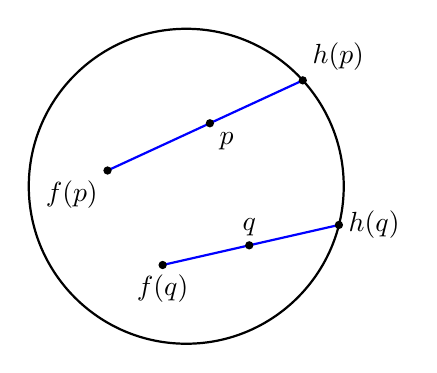
\begin{tikzpicture}
\draw[thick] (0,0) circle (2);
\coordinate (fp) at (-1.0,0.2);
\coordinate (p) at (0.3,0.8);
\coordinate (hp) at (1.480,1.345);
\coordinate (fq) at (-0.3,-1.0);
\coordinate (q) at (0.8,-0.75);
\coordinate (hq) at (1.9388,-0.4912);
\draw[blue, thick] (fp) -- (hp);
\draw[blue, thick] (fq) -- (hq);
\foreach \pt in {fp,p,hp,fq,q,hq} \fill (\pt) circle (1.5pt);
\node[below left] at (fp) {$f(p)$};
\node[below right] at (p) {$p$};
\node[above right] at (hp) {$h(p)$};
\node[below] at (fq) {$f(q)$};
\node[above] at (q) {$q$};
\node[right] at (hq) {$h(q)$};
\end{tikzpicture}
